\documentclass[intern,palatino]{cgBA}

\author{Sebastian Gaida}
\title{Simulation von Rauch}
\zweitgutachter{Bastian Krayer MSc. }
\zweitgutachterInfo{(Institut für Computervisualistik, AG Computervisualistik)}
\externLogo{7.46cm}{logos/UniLogoNeu}
\externName{DIN: NewTechnologies}

\sloppy

\usepackage{acronym}
\usepackage{hyperref}
\usepackage{url}
\usepackage{listings}
\usepackage{xcolor}
\usepackage{float}

\lstset{language=C++,
	frame=tb,
	tabsize=4,
	showstringspaces=false,
	numbers=left,
	commentstyle=\color{olive},
	keywordstyle=\color{blue},
	stringstyle=\color{red}
}

\setcounter{secnumdepth}{4}

\begin{document}

	\maketitle
	\newpage
	\pagenumbering{roman}
	\tableofcontents
	\clearpage         % oder \cleardoublepage bei zweiseitigem Druck
	% \listoffigures   % fuer ein eventuelles Abbildungsverzeichnis
	\pagenumbering{arabic}
	\bibliographystyle{alphadin}

%-------------------------------------------------------------------------------

\section*{Abstract}\label{abstract}

In dieser Arbeit wird auf die realistische Simulation von Rauch eingegangen. Dabei bezieht sich die Arbeit hauptsächlich auf die Simulationen von Müller et al.\cite{muller2003particle} und Ren et al.\cite{ren2016fast}. Die Simulation wurde mittels C++, der OpenGL und Compute-Shadern erstellt. Hierbei wurde das SPH-Verfahren genutzt und die Möglichkeiten zur Beschleunigung auf der GPU untersucht.
\newline \newline
This paper deals with the realistic simulation of smoke. The work refers mainly to the simulations of Müller et al.\cite{muller2003particle} and Ren et al.\cite{ren2016fast}. The simulation was created using C++, the OpenGL and compute shaders. Here the SPH method was used and the possibilities to accelerate it on the GPU were investigated.
\newpage

%-------------------------------------------------------------------------------

\section{Vorwort}\label{vorwort}

Vor dem Beginn der vorliegenden Bachelorarbeit möchte ich mich zunächst bei einigen Personen bedanken die mich während der Arbeit unterstützt haben.
\newline \newline
Zunächst einmal bedanke ich mich bei Prof. Dr.-Ing. Stefan Müller und Bastian Krayer MSc. für die großartige Betreuung meiner Arbeit.
\newline
Außerdem möchte ich mich bei Pascal Bendler bedanken, der mich tatkräftig beim debugging unterstützt hat.
\newline
Ein großes Dankeschön geht auch an den Freund, der mich immer wieder dazu motiviert hat weiter zu arbeiten und nach alternativen Möglichkeiten zu suchen.
\newpage

%-------------------------------------------------------------------------------

\section{Einleitung}\label{einleitung}

Das Ziel dieser Arbeit ist es eine möglichst physikalisch korrekte Rauchsimulation zu implementieren. Dazu nutzen wir, dass sich Rauch wie ein Fluid verhält \cite{stam2003real}, dabei wird die Simulation der physikalischen Basis von Fluiden angenähert. Hierbei wird in dieser Implementation ein Partikelsystem zur Berechnung der physikalischen Eigenschaften genutzt. Echtzeitanwendungen wie die Unity-Engine bieten eine Partikelsimulation an, jedoch beschränkt sich diese lediglich auf das Ausstoßen von Partikeln. Dabei können Partikelinteraktionen, sowie Verhaltensmuster nicht bearbeitet werden.
\newline \newline
Die GPU eignet sich besonders gut zum berechnen parallelisierbarer Rechenoperationen, da sie im Vergleich zur CPU, die nur wenige Kerne besitzt, über tausend Kerne verfügt, die zwar nicht so leistungsfähig sind wie die der CPU, aber dennoch einen signifikante Steigerung der Leistung bieten.
\newline \newline
In der Arbeit wird auch darauf eingegangen den genannten Aufwand zu minimieren, dazu wurden zwei Verfahren zur Beschleunigung des Partikelsystems, auf der GPU,  implementiert und gegenübergestellt.
\newline \newline
Für die Implementation wurde OpenGL genutzt, welches das programmieren auf der GPU deutlich vereinfacht und seit der Version 4.3 auch das verarbeiten von Daten mit Hilfe von Compute-Shadern unterstützt. Für den schnellstmöglichen Zugriff auf diese Daten wird Speicherplatz, in Form von SSBO, auf derGPU angelegt. Dabei sollte auch auf eine effiziente Nutzung des limitierten Speicherplatzes geachtet werden.

%-------------------------------------------------------------------------------

\section{State of the Art}\label{state}
Die Simulation von einem Systemen, zur Darstellung von Fluiden, ist ein jahrelange Herausforderung für die Computergrafik. Dabei treten immer wieder die gleichen Problemstellungen auf. Zum einen soll die Simulation physikalisch korrekt sein, um eine für den Beobachter ein möglichst schönes, sowie nachvollziehbarer Ergebnis zu bieten. Schon kleinstes Fehlverhalten können die Immersion zerstören. Andererseits soll das System auch in Echtzeit berechnet werden und dabei auf mögliche Interaktionen reagieren können. Für eine möglichst effiziente Berechnung werden verschiedene Beschleunigungsverfahren verwendet, die ein gutes Ressourcenmanagement in Form der Laufzeit sowie Speicherplatz erfordern.
\newline \newline
Die physikalische Grundlage, die Navier-Stokes-Gleichungen, basiert dabei auf den Gleichungen die von Claude Louis Marie Henri Navier und George Gabriel Stokes im 19. Jahrhundert aufgestellt wurden \cite{wiki:xxx}. Diese Gleichungen beschreiben die physikalischen Eigenschaften von Fluiden und werden für die Simulation dieser angewendet. Diese Formeln werden je nach Fluid noch angepasst um speziellere Eigenschaften darzustellen.
\newline
Diese Simulation wird meist in Form eines rasterbasierenden Verfahren oder eines Partikelsystems implementiert.\newline

%-------------------------------------------------------------------------------

\subsection{Vektorfeldverfahren}\label{vektor}
Beim Vektorfeldverfahren wird die Umgebung in gleichgroße Voxels unterteilt, auch bekannt als Voxelgrid oder eulersches Grid. Bei diesem Vektorfeldverfahren betrachtet man die Partikel nicht direkt sondern einen Masse die in Form des Voxels generalisiert wird. Dabei werden Parameter wie Dichte, Druck und Geschwindigkeit in dem jeweiligen Voxel gespeichert. Die Berechnungen lassen sich in Advektion, Druck, Diffusion und Beschleunigung unterteilen. Die Advektion beschreibt dabei den Strömungstransport, das Übertragen der Bewegungskraft auf ein anliegendes Objekt. Druck wiederum beschreibt die Übertragung von Kräften an benachbarte Partikel, wodurch bei einem zu hohen Druck eine Kraft vom Zentrum weg entsteht und wiederum bei einem Unterdruck eine Kraft zum Zentrum hin. Die Diffusion beschreibt die Viskosität des Fluides. Je nach Anpassung der breitet sich das Fluid stark aus wie zum Beispiel Wasser oder weniger stark wie Lava aus.
Bei Beschleunigung handelt es sich um externe Kräfte die auf das Fluid einwirken, dies ist vergleichbar mit der Schwerkraft oder einer Windgeschwindigkeit. Zur Beschleunigung zählt man bei den Vektorfeldern aber auch die Wirbelkraft, die bei Rauch die typischen Turbulenzen verursacht und damit einen signifikanten Einfluss auf die Erscheinung hat.
\newline
Wegen der physikalisch präziseren Ergebnisse eignet sich diese Verfahren besonders für Strömungsimulationen in Innenräumen \cite{franz}, da man Kraft dem System zuführt, diese Kraft wird daraufhin eingefärbt und spiegelt dabei das Fluid wieder.
\newline
Bei dieser Methode stellt das Lösen der Gleichungen und die Visualisierung der Ergebnisse die größte Schwierigkeit da. Die Visualisierung erweist sich als Hindernis, da in jedem Voxel Kräfte vorhanden sind. Dabei unterscheidet man in dem Grid unter einem gefärbten Teil und einem nicht sichtbaren Teil der meist Luft repräsentiert \ref{img:Vertexfeld}. Zur Darstellung des Fluides wird meist Volumerendering genutzt. Außerdem ist, wegen der Grid-Architektur des Verfahrens, der Rechenaufwand hoch und lässt sich nur schwer verbessern.

\begin{figure}[h]
	\centering
	\includegraphics[width=0.7\columnwidth]{Bilder/vektorfeld.jpg}
	\caption[Fluidsimulation in Form des Vektorfeldverfahren \newline Quelle:\url{https://thumbs.gfycat.com/CelebratedElasticHartebeest-poster.jpg}]{Fluidsimulation in Form des Vektorfeldverfahren}
	\label{img:Vertexfeld}
\end{figure}

%-------------------------------------------------------------------------------

\subsection{Partikelsystem}\label{partikel}

Bei dem Verfahren einer Partikelsimulation werden die Partikel einzeln betrachtet, dies bezeichnet man auch lagrangiansches Verfahren. Diese speichern Parameter wie Position und Geschwindigkeit selber ab. Die Berechnungen beschränken sich dabei auf die Dichte, Druck, Viskosität, Auftrieb und Wirbelkraft.
Bei den Berechnungen werden die Nachbarpartikel mit einbezogen. Die Dichte beschreibt dabei wie viele Nachbarpartikel Einfluss auf dieses bestimmte Partikel haben und wird als Gewichtung für die Berechnung der Kräfte verwendet. Das typische Verhalten des Fluides, wird aber durch das Zusammenspiel der Kräfte Drucke und Viskosität erzeugt. Dabei sorgt der Druck dafür, dass Partikel sich voneinander wegbewegen und die Viskosität wirkt dem entgegen und führt das Anziehen von Partikel hervor. Der Auftrieb wiederum lässt sich über die Temperatur des Rauches bestimmen, welche je nach Dichte steigt oder sinkt. Zum anderen lässt sich aber die Wirbelkraft nicht so einfach berechnen und stellen somit ein Problem in der Forschung dar.
Für die Berechnungen werden die Nachbarpartikel benötigt, welche aber nicht für jeden Partikel bekannt sind und es entsteht ein großer Aufwand, wenn man aus Einfachheit alle Partikel mit einbezieht. Hierbei entstehen viele Möglichkeiten das System zu beschleunigen.
\newline
Der Ansatz eines Partikelsystems eignet sich hervorragen zum einbinden in eine Echtzeitanwendung, wie ein Computerspiel oder einer Engine, da man mit der Partikelanzahl  die Performance beeinflussen kann. Beim Reduzieren der Partikel sollte eine Anpassung der Parameter erfolgen, da dies sonst einen signifikanten Einfluss auf das Verhalten des Fluides hat.
\newline
Die größten Schwierigkeiten bei einer Rauchsimulation in Form eines Partikelsystems entstehen durch Beschleunigung der Nachbarschaftssuche, sowie den Auftrieb und die Wirbelkraft.
\begin{figure}[h]
	\centering
	\includegraphics[width=0.7\columnwidth]{Bilder/partikelsystem.jpg}
	\caption[Partikelsimulation von Wasser \newline \url{https://i.ytimg.com/vi/DhNt_A3k4B4/maxresdefault.jpg}]{Partikelsimulation von Wasser}
	\label{img:Partikelsystem}
\end{figure}

%-------------------------------------------------------------------------------

\section{Rauchsimulation}\label{rauch}

% Längeren Text
Zur Simulation von Rauch wurde ein Partikelsystem implementiert, wessen physikalische Grundlage auf dem SPH-Verfahren basiert, welches Müller \cite{muller2003particle} 2003 zur Simulation von Fluiden genutzt hat. Dabei handelt es sich um eine Abwandelung der Navier-Stokes-Gleichungen für die Berechnung der Dichte, Druckes und Viskosität. Diese wurden zur Verwendung in einem SPH angepasst. Der Auftrieb, sowie die Temperaturberechung, stammen aus einem Paper von Ren \cite{ren2016fast}. Die größten Probleme bei der Implementation bereitete aber die Wirbelkraft, Ren und Macklin \cite{macklin2014unified} boten eine Formel zur Berechnung dar, welche aber nicht das gewünschte Ergebnis lieferte.
\newline
Die Berechnung der Simulation bedarf vieler Schritte die von einander abhängig sind. In Abbildung  \ref{code:sim} werden alle Rechenschritte in einen optimalen Reihenfolge dargestellt. Die Berechnungen lassen sich in 4 Compute-Shader unterteilen.
\newline
Zum Verständnis bildet Abbildung \ref{tab:Symbole} alle Variablen da, sowie deren Bedeutung und Format.

%todo überarbeiten

\begin{figure}
	\centering
	\begin{lstlisting}
computeshader 1	
	for all particle i do
		for all neighbor of i do
			calculate density
		end for
		calculate pressure
	end for
end computeshader 1
computeshader 2
	for all particle i do
		for all neighbor of i do
			calculare normal
		end for
		calculate vorticity
	end for
end computeshader 2
computeshader 3
	for all particle i do
		for all neighbor of i do
			calculate pressure force
			calculate viscosity force
			calculate vorticity force
			calculate temperature
		end for
		calculate temperature cooldown
		calculate buoyancy force
		update velocity
	end for
end computeshader 3
computeshader 4
	for all particle i do
		apply velocity on position
	end for
end computeshader 4
	\end{lstlisting}
	\caption{Updateschleife der Physik}
	\label{code:sim}
\end{figure}

\begin{figure}
	\centering
		\begin{tabular}{ | c | p{8cm} | c |}
			\hline
			Symbol & Bedeutung & Format  \\ \hline
			$m_i $ 				&  Masse des Partikel i								&	float	\\ \hline
			$r_i $		 		&  Position des Partikel i							&	vec3	\\ \hline
			$r_{ij}$ 			&  Abstandsvektor von $r_i - r_j$					&	vec3	\\ \hline
			$v_i$	 			&  Geschwindigkeitsvektor des Partikel i			&	vec3	\\ \hline
			$h $ 				&  Radius											&	float	\\ \hline
			$W_{ij} $ 			&  Gewichtungsfunktion, kurz für $W (r_i - r_j)$	&	float	\\ \hline
			$\nabla W_{ij} $ 	&  Gradienten-Gewichtungsfunktion					&	vec3	\\ \hline
			$\nabla^2 W_{ij} $ 	&  Laplace-Gewichtungsfunktion						&	float	\\ \hline
			$\rho_i $ 			&  Dichte des Partikel i		 					&	float	\\ \hline
			$\rho_0 $ 			&  Ruhedichte im Allgemeinen						&	float	\\ \hline
			$k $ 				&  Steifheit des Fluides							&	float	\\ \hline
			$p_i $ 				&  Druck des Partikel i								&	float	\\ \hline
			$f^{pressure}_i $	&  Druckkraft des Partikel i						&	vec3	\\ \hline
			$\mu $ 				&  Viskosität des Fluides							&	float	\\ \hline
			$\nu_i $ 			&  Viskosität des Partikel i						&	float	\\ \hline
			$f^{viscosity}_i $ 	&  Viskositätskraft des Partikel i					&	vec3	\\ \hline
			$T_i $ 				&  Temperatur des Partikel i						&	float	\\ \hline
			$D_r $ 				&  Zeit zum halbieren der Temperatur				&	float	\\ \hline
			$b $ 				&  Up-Vektor										&	vec3	\\ \hline
			$D_c $ 				&  Wärmeleitfähigkeitsfunktion des Fluides			&	float	\\ \hline
			$c $ 				&  Wärmeleitfähigkeit								&	float	\\ \hline
			$C_b $ 				&  Auftriebs-Koeffizient							&	float	\\ \hline
			$a_{b,i} $ 	  		&  Auftriebsbeschleunigung							&	vec3	\\ \hline
			$n_i $ 				&  Normale des Partikel i							&	vec3	\\ \hline
			$C_N $ 				&  nutzerdefinierter Schwellenwert					&	float	\\ \hline
			$y $ 				&  Zahl die nahezu 0 ist					 		&	float	\\ \hline
			$f^{buoyancy}_i $ 	&  Auftriebskraft des Partikel i					&	vec3	\\ \hline
			$\beta $ 			&  nutzerdefinierter Wert							&	float	\\ \hline
			$\omega_i $ 		&  Wirbelstärke des Partikel i						&	vec3	\\ \hline
			$f^{vortex}_i $ 	&  Wirbelkraft des Partikel i						&	vec3	\\ \hline
			$g $ 				&  Gravitationskraft								&	vec3	\\ \hline
			$ext $ 				&  externe Kraft									&	vec3	\\ \hline
			$\delta t $ 		&  Zeit seit letzter Iteration 						&	float	\\ \hline
			$\delta $ 			&  veränderte Wert im Abstand von $\delta t$ 		&			\\
			\hline
		\end{tabular}
	\caption{Bedeutung aller Symbole der Berechnungen}
	\label{tab:Symbole}
\end{figure}

%-------------------------------------------------------------------------------

\subsection{Gewichtungsfunktionen}\label{kernel}

Ein wichtiger Aspekt welchen Einfluss Nachbarpartikel auf den betrachteten Partikel haben sind die Gewichtungsfunktionen. Diese bestimmen den Einfluss über die Entfernung $r_{ij}$ der Partikel zu einander, dabei spielt der Radius als Maximalabstand eine wichtige Rolle. Die Funktionen besitzen alle die Eigenschaft, dass sie symmetrisch sind und beim erreichen des Radius gegen 0 konvergieren und damit haben weit entfernte Partikel keinen Einfluss mehr. Gewichtungsfunktionen dienen dazu um eine Stabilität in das Partikelsystem zu bringen. Dabei nähern sie sich üblich Ableitungen von bestimmten Funktionen an \cite{muller2003particle}. Diese Funktionen wurden mit Hilfe von Bastian Krayer implementiert.
\newline
Für das SPH werden die drei folgenden Gewichtungsfunktionen genutzt. Abhängig von den Berechnungen wird eine andere Funktion für die richtige Stabilität des Systems benötigt. In Abbildung \ref{img:kernel} ist der Verlauf der Funktionen dargestellt.
\newline
Die $W_{poly}$-Funktion \ref{funk:normal} bietet einen weichen abfallenden Verlauf bei ansteigendem Abstand, diese Funktion wird als Standard für jegliche Berechnung genutzt.
\newline
Es werden aber für die Berechnungen ebenfalls ein Gradient, sowie der Laplace benötigt. Der Gradient für die Druckberechnung lässt sich durch die Ableitung der für diese Berechnung vorgesehene Funktion berechnen. Mit der $W_poly$-Funktion beim Wert 1, bei der die Druckkraft am höchsten sein sollte, ein nahezu 0 Wert erreicht, welcher dazu führen würde, dass sehr nahe Partikel sich nicht mehr abstoßen würden. Deshalb nutzt Müller Desbrun \cite{desbrun1996smoothed} Funktion \ref{funk:gradient}, da diese in der Ableitung \ref{funk:gradient2} Werte liefert, die für die Berechnung entsprechend konvergieren.
\newline\newline

\begin{equation}\label{funk:normal}
	W_{poly6}(r_{i,j}) = \frac{315}{64 \pi h^9}   
	\begin{cases}
	(h^2 - r^2)^3 		& 0	\leq r \leq h	\\
	0					& otherwise			\\
	\end{cases}
\end{equation}

\begin{equation}\label{funk:gradient}
W_{spiky}(r_{i,j}) = \frac{15}{\pi h^6}   
\begin{cases}
(h - r)^3 		& 0	\leq r \leq h	\\
0					& otherwise			\\
\end{cases}
\end{equation}

\begin{equation}\label{funk:gradient2}
\nabla W_{spiky}(r_{i,j}) = \frac{-45}{\pi h^6}   
\begin{cases}
(h - r)^2 		& 0	\leq r \leq h	\\
0					& otherwise			\\
\end{cases}
\end{equation}

\begin{equation}\label{funk:laplace}
W_{visc}(r_{i,j}) = \frac{15}{2 \pi h^3}   
\begin{cases}
-\frac{r^3}{2h^3} + \frac{r^2}{h^2} + \frac{h}{2r} -1  		& 0	\leq r \leq h	\\
0					& otherwise			\\
\end{cases}
\end{equation}

\begin{equation}\label{funk:laplace2}
\nabla ^2 W_{visc}(r_{i,j}) = \frac{45}{\pi h^6}
\begin{cases}
(h-r) 		& 0	\leq r \leq h	\\
0					& otherwise			\\
\end{cases}
\end{equation}

\newpage

\begin{figure}[h]
	\centering
	\includegraphics[width=0.7\columnwidth]{Bilder/kernel.jpg}
	\caption{Die Gewichtungsfunktionen $W_{poly6}$, $W_{spiky}$, $W_{visc}$ nach \cite{muller2003particle} mit einem Radius von 1}
	\label{img:kernel}
\end{figure}
Die $W_{spiky}$-Funktion, würde aber wiederum in der zweiten Ableitung 0 werden, bei anderen standardmäßigen Gewichtungsfunktionen könnte es sogar dazu führen, dass ein negativer Wert auftritt, der bei der Viskosität einen gegensätzlichen dem gewünschtem Effekt hätte. Deshalb wurde die $W_{visc}$-Funktion \ref{funk:laplace} entworfen, dessen Laplace \ref{funk:laplace2} optimal für die Berechnung der Viskosität ist.

\begin{figure}[H]
	\centering
	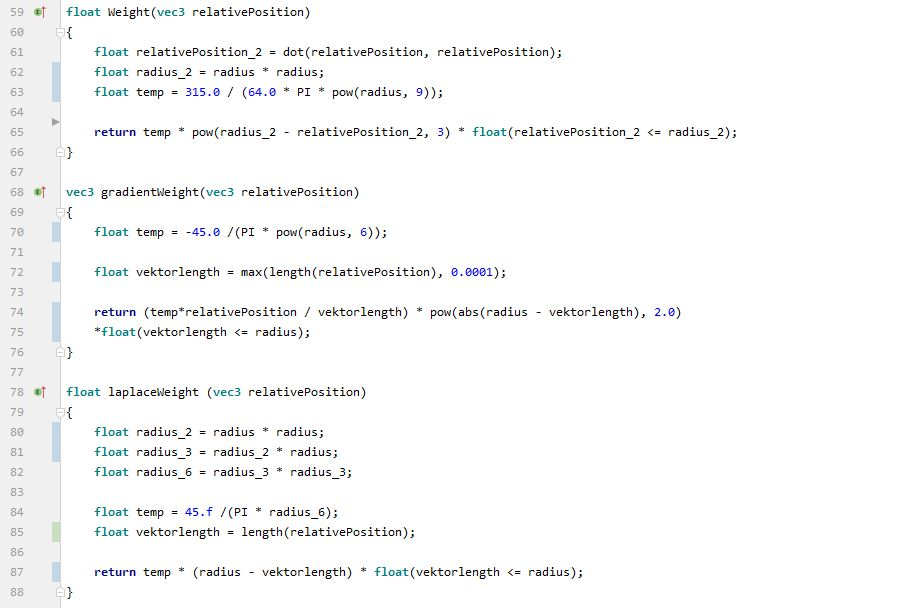
\includegraphics[width=1.35\columnwidth]{Bilder/impKernel.jpg}
	\caption{Implementation der SPH Kernel}
	\label{img:impkernel}
\end{figure}

In Abbildung \ref{img:impkernel} sind die Implementationen dargestellt. Dabei handelt es sich um die Funktionen $W_{poly6}$ in Zeile 59, $\nabla W_{spiky}$ in Zeile 68 und $\nabla^2 W_{visc}$ in Zeile 78.\newline
Die Abbruchfunktionen, wie in \ref{funk:normal}, \ref{funk:gradient2} und \ref{funk:laplace2} zu sehen, wurden dabei durch die Multiplikation mit einer boolesche Variable durchgeführt, welche bei einem Abstand höher als dem Radius dazuführt, dass das Ergebnis 0 wird.

%-------------------------------------------------------------------------------

\subsection{Dichte}\label{dichte}

Die Dichte ist eine Variable die für jeden Partikel individuell berechnet wird. Sie beschreibt die Anzahl der Partikel in unmittelbarer Nähe. Außerdem wird sie bei fast jeder folgenden Berechnung benötigt, da sie als Gewichtung des eingenommenen Volumens dient. 

\begin{equation}\label{funk:skalar}
A_s(r_i) = \sum_j m_j \frac{A_j}{\rho_j} W(r_i-r_j)
\end{equation}
\begin{equation}\label{funk:density}
\rho_i(r_i) = \sum_j m_j \frac{\rho_j}{\rho_j} W(r_i-r_j) = \sum_j m_j  W(r_{i,j})
\end{equation}

Die Dichte, wie in der Gleichung \ref{funk:density} zu sehen, errechnet sich aus der Summe über alle Nachbarn j. Dabei multiplizieren wir die Masse $m_j$ mit der Dichte $\rho_j$ durch die Dichte. Dies wird dann noch mit der Gewichtungsfunktion verrechnet. Die Gleichung ergibt sich aus der Berechnung für Skalaregrößen \ref{funk:skalar} von Müller \cite{muller2003particle}.
\newline\newline
Wie in Abbildung \ref{img:dichte} Zeile 90 zu sehen, ist die Masse der Partikel nicht vom jeweiligen Partikel abhängig. In dem Paper von Ihmsen \cite{ihmsen2014sph} wird eine Formel $m_i = h^3 \rho_0$ für die Masse vorgestellt, diese wird initial durchgeführt und die Masse ist für den Rest der Simulation gleichbleibend. Diese Formel hat sich aber als nicht stabil, in der Implementation, herausgestellt. Deshalb wurde sie als Uniform-Variable implementiert die bei allen Partikel gleich ist. Der Vorteil dieser Implementation ist, dass man die Masse zu beginn oder auch zur Laufzeit verändern kann. Wobei dem ändern während der Laufzeit abzuraten ist, da es zu einem instabilen Verhalten der Simulation führen kann.
\newline
In Zeile 87-89 ist ein If-Abfang eingebaut der es verhindert, dass die Partikel auf sich selbst Einfluss nehmen können. Auf die Begrenzung der Nachbarn, die in die Berechnung eingenommen werden, wird in Abschnitt \ref{besch} eingegangen.
\begin{figure}[H]
	\centering
	\includegraphics[width=1.35\columnwidth]{Bilder/dichte.jpg}
	\caption{Implementation der Dichtefunktion}
	\label{img:dichte}
\end{figure}

%-------------------------------------------------------------------------------

\subsection{Druck}\label{druch}

Der Druckkraft $f^{pressure}$ beschreibt das Abstoßen von Partikeln von einander. Die standardmäßige Berechnung für Skalaregrößen \ref{funk:skalar}, ist aber in diesem Fall nicht symmetrisch und würde zu einen instabilen Simulation führen. Da für Partikel i nur der Druck $p$ des Nachbarpartikel j relevant wäre. Dies würde zu einem unterschiedlichen Druckkraft bei der Berechnung des Druckes zwischen den zwei Partikeln führen. Um dieses Problem zu umgehen stellt Müller \cite{muller2003particle} eine alternative Formel \ref{funk:pressureF} vor, die eine symmetrische Berechnung zwischen den Partikeln ermöglicht. Dabei werden beide Druckwerte addiert, um das Verhältnis aber beizubehalten wird auch die Dichte im Nenner verdoppelt. Zur Gewichtung wird dabei die Gradientenfunktion \ref{funk:gradient2} genutzt und damit der Vektor vom anderen Partikel j weg zeigt wird dieser negiert.
\newline
Zum berechnen der Druckkraft muss aber zunächst der Druck berechnet werden. Die Formel \ref{funk:pressure} von Desbrun \cite{desbrun1996smoothed} diesbezüglich wurde angepasst, indem eine Ruhedichte von der eigentlichen Dichte abgezogen wird. Dabei wird die Ruhedichte $p_0$ als Offset verwendet und hat keinen mathematischen Einfluss auf die Druckkraft \cite{muller2003particle}. Die Variable $k$ beschreibt dabei die Steifheit und bestimmt wie stark sich der Rauch ausdehnt.

\begin{equation}\label{funk:pressure}
p_i = k(\rho - \rho_0)
\end{equation}
\begin{equation}\label{funk:pressureF}
f^{pressure}_i = - \nabla p(r_i) = - \sum_j m_j \frac{p_i+p_j}{2\rho_j} \nabla W(r_{i,j})
\end{equation}

%-------------------------------------------------------------------------------

\subsection{Viskosität}\label{visc}

Ein wichtiger Aspekt der Physik ist auch die Viskosität. Diese beschreibt den Einfluss der Kraft der umliegenden Partikel, dabei haben aber nicht alle Partikel gleich viel Einfluss auf einander. Dies resultiert daraus, dass die Viskosität eine asymmetrische Kraft ist.   Wäre sie jedoch eine symmetrische Kraft würde es dazuführen ,dass viele Partikel die alle gleichzeitig in eine Richtung bewegen, sich ins unendliche beschleunigen würden. Dabei würde es bereits reichen, dass ein einzelner Partikel seine Kraft überträgt, da dieser wie bei einem Dominoeffekt, alle Partikel in seiner Umgebung in seine Bewegungsrichtung beschleunigen würde. Um dies zu umgehen modifiziert Müller \cite{muller2003particle} die SPH-Formel \ref{funk:skalar} indem der Unterschied des Geschwindigkeitsvektor $v$ in Betracht gezogen wird. Dies sorgt dafür, dass ein Partikel mit einem großen Geschwindigkeitsvektor trotzdem noch alle Partikel in seiner Nähe mit sich reißt, aber sich nicht mehr ins unendliche beschleunigen kann.
\newline
Dies lässt den Rauch wirken als würde er sich zusammen ziehen. Das resultiert daraus, dass die Partikel, mit der angepassten Formel, sich auch abbremsen können, da ein schnellerer Partikel beim berechnen der Viskosität mit einem langsamen Partikel einen Viskositätskraft entgegen seiner Bewegungsrichtung erhält. 
\newline
Wie in \ref{funk:visc} wird der Geschwindigkeitsvektor des eigenen Partikel abgezogen. Als Gewichtungsfunktion wird dabei der Laplace\ref{funk:laplace2} der $W_{visc}$\ref{funk:laplace} genutzt.

\begin{equation}\label{funk:visc}
f^{visc}_i  = \mu \sum_j m_j \frac{v_j-v_i}{\rho_j} \nabla^2 W(r_{i,j})
\end{equation}

Die Variable $\mu$ beschreibt die eigentliche Viskosität. $\mu$ ist bei Fluiden wie Honig hoch und bei Rauch sehr gering. In der Implementation hat $\mu$ deshalb einen Wert von $0.25$.

%-------------------------------------------------------------------------------

\subsection{Auftrieb}\label{auftrieb}

Auftrieb ist eine Kraft die abhängig von der Temperatur des Rauches ist. Oftmals wird diese Temperatur statisch implementiert und sich eine Berechnung dieser gespart. Dabei zu beachten ist, dass die Partikel sich bei einer hohen Dichte gegenseitig aufheizen und bei einer niedrigen abkühlen. Um dieses Verhalten umzusetzen wurde die Auftriebsvariante von Ren \cite{ren2016fast} implementiert.
\newline
Zum anpassen der Temperatur der Partikel wurde die Formel \ref{funk:temp} verwendet. Diese betrachtet die Nachbarpartikel und heizt bzw. kühlt die Partikel abhängig der Nachbarn auf oder ab. Bei dieser Formel fehlte aber eine Definition der Funktion Dc, weshalb diese durch die in \ref{imp:temp} ersetzt wurde. Diese multipliziert den Temperatur unterschied mit einer Konstanten $C$ die den Wärmestrom des Rauches beschreibt. $\gamma$ ist dabei nur eine Variable, die positiv und nahe $0$ist, die das Teilen durch $0$ verhindert.
\newline
Die Formel \ref{funk:temp2} beschreibt zudem das Abkühlen von Partikeln die kaum bis keine Nachbarpartikel haben. Dafür wird die Temperatur durch die Zeit geteilt die benötigt wäre um die Temperatur zu halbieren. Welche Partikel dabei betroffen sind wird über die Normale $n_i$ ermittelt, dazu wird die Formel \ref{funk:normale} verwendet. Die Normale wird bei einer geringen Dichte $\rho$ größer und wenn diese einen nutzerdefinierten Schwellwert überschreitet führt dies zur Abkühlung des Partikel. Leider lässt sich diese Formel nur bei einer positiven Temperatur anwenden, welches das Abkühlen von bereits negativen Temperatur verhindert.
\newline
Wenn die Temperatur errechnet wurde lässt diese sich wie in \ref{funk:temp3} berechnen. Dabei beschreibt $b$ einen Up-Vektor und $C_b$ den Auftriebs-Koeffizienten.

\begin{equation}\label{funk:temp}
\frac{\delta T_i}{\delta t}  = \sum_j \frac{m_j}{\rho_i \rho_j} Dc(T_i - T_j) \frac{(r_i-r_j) \cdot \nabla W_{i,j}}{(r_i-r_j)^2 + \gamma^2}
\end{equation}

\begin{equation}\label{funk:normale}
n_i  = \sum_j \frac{m_j}{\rho_j} \nabla W_{i,j}
\end{equation}

\begin{equation}\label{funk:temp2}
\frac{\delta T_i}{\delta t}  = - T_i/D_r
\end{equation}

\begin{equation}\label{funk:temp3}
f^{buoyancy}_i  = C_b T_i b
\end{equation}


\begin{figure}[H]
	\centering
	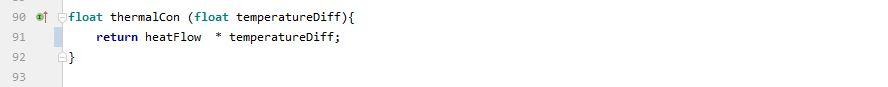
\includegraphics[width=1.35\columnwidth]{Bilder/thermal.jpg}
	\caption{Implementation der Wärmeleitfähigkeit}
	\label{img:temp}
\end{figure}

%-------------------------------------------------------------------------------

\subsection{Wirbelkraft}\label{wirbel}

Die Wirbelkraft ist die schwierigste zu berechnende Kraft in einem SPH. In dem Paper von Ren \cite{ren2016fast} wird eine beschrieben und ebenfalls die von Macklin \cite{macklin2014unified} erwähnt.
\newline
Ein Bestandteil der Wirbelkraft ist die Wirbelstärke, die sich aus dieser und dem Geschwindigkeitsgradienten, sowie der Normalen und der Gravitation errechnen lässt \ref{funk:wirb}. Bei dem Geschwindigkeitsgradienten ist aber zu beachten, dass dieser eine Jacobi-Matrix der Geschwindigkeit ist und dort eine Matrixmultiplikation mit der Wirbelstärke stattfindet. Um den Gradienten anzunähern wird wie von Macklin \cite{macklin2014unified} empfohlen ein SPH-Gewichtungsfunktion \ref{funk:gradient2} zu nutzen. Diese Formel beschreibt den Abstand des Partikel zu der Oberfläche des Rauches, dabei repräsentiert ein hoher Wert die Oberflächenpartikel und ein kleiner die inneren Partikel.
In der Formel \ref{funk:wirb2} wird dann noch die Wirbelstärke der umliegenden Partikel mit dem Abstandsvektor als Vektorprodukt verrechnet, um einen Vektor zu erhalten der eine Verwirbelung innerhalb des Fluides verursachen soll.  
\begin{equation}\label{funk:wirb}
\frac{\delta \omega_i}{\delta t}  = \omega_i \cdot + \nabla v + \beta(n_i \times g)
\end{equation}

\begin{equation}\label{funk:wirb2}
f^{vortex}_j  = \sum_j (\omega_j \times (r_i -r_j)) W_{i,j}
\end{equation}

Eine Wirbelkraft zu errechnen die Turbulenzen verursacht ist leider nicht gelungen. Diese hatte lediglich die Wirkung die, dass der Rauch langsamer aufgetrieben ist. 

%-------------------------------------------------------------------------------

\subsection{Update Kräfte}\label{kräfte}

Abschließend werden alle Kräfte zusammen gerechnet und zum Geschwindigkeitsvektor hinzugefügt \ref{funk:update}. Ein Spezialfall dabei ist die Gravitation die mit der Dichte verrechnet wird. Zusätzlich können auch externe Kräfte $ext$ hinzugefügt werden um bestimmte Umwelteinflüsse zu simulieren. Dabei beschränkt es sich lediglich auf einen Vektor der bei allen Partikeln gleichstark wirkt.
\newline

\begin{equation}\label{funk:update}
\frac{\delta v_i}{\delta t}  = f^{pressure}_i + f^{viscosity}_i + f^{buoyancy}_i + f^{vortex}_i + ext + \rho_i g
\end{equation}

\begin{figure}[H]
	\centering
	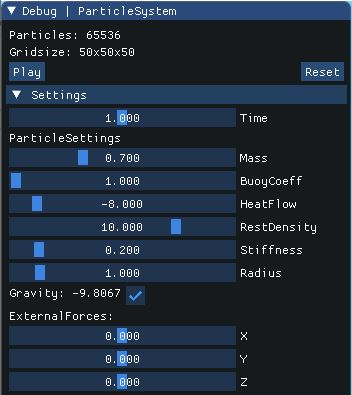
\includegraphics[width=0.35\columnwidth]{Bilder/external.jpg}
	\caption{Anpassbare Variablen per ImGui}
	\label{img:ext}
\end{figure}
\newpage

%-------------------------------------------------------------------------------

\section{Implementierung}\label{imp}

Bei der Implementierung wurde darauf geachtet, dass das System einfach und schnell anpassbar ist um das Testen zu vereinfachen.
Dazu können einige Parameter während der Laufzeit angepasst werden. Hierfür wurde ImGui \cite{ocornut} verwendet, welches eine UI \ref{img:ext} zur Verfügung stellt um die Parameter anzupassen.
Das Anpassen der Variablen während der Laufzeit kann aber zur Instabilität der Physik führen.
\newline
Da die Implementierung die GPU verwendet muss darauf geachtet werden, dass die angewendeten Verfahren auch parallel berechenbar sind. Da nicht alle Kerne der GPU gleich schnell arbeiten muss es verhindert werden, dass Werte die von anderen Prozessen noch gelesen wird nicht überschrieben werden.
Um dieses Problem zu umgehen wurden zwei identische SSBOs für die Partikel angelegt, welches zwar mehr Speicheraufwand bedeutet, aber bei ca. 65.000 Partikel nur zusätzlich 12 KB beträgt. Bei den zwei SSBOs werden diese im wechsel zum lesen un schreiben genutzt \ref{img:flipflop}. Dadurch besitzt das lesbare SSBO die zuletzt berechneten Daten und schreibt die neuen in das beschreibbare SSBO, hierbei wird aber immer anfangs das beschreibbare zunächst mit dem lesbaren SSBO überschrieben, damit alle Daten aktuell sind.
Es muss dabei aber auch auf eine gerade Anzahl der aufrufe der Compute-Shader geachtet werden, da sonst im Beginn der Update-Schleife aus dem falschen SSBO gelesen wird.
\newline
%todo ergänzen atomicOperationen 

\begin{figure}[H]
	\centering
	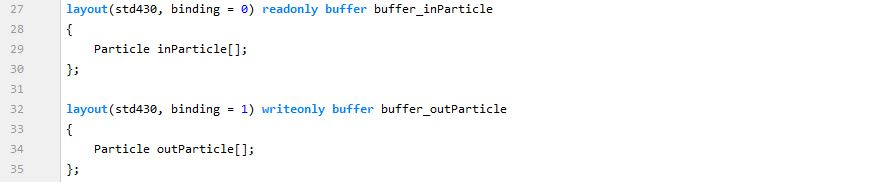
\includegraphics[width=1.3\columnwidth]{Bilder/Flipflop.jpg}
	\caption{Partikel SSBOs zum lesen und schreiben}
	\label{img:flipflop}
\end{figure}
\newpage
%-------------------------------------------------------------------------------

\section{Beschleunigung}\label{besch}

Um ein Partikelsystem in einer Engine zu integrieren, muss diese möglichst performant sein, da in einer Engine auch andere Prozesse berechnet werden. Es bestehen mehrere Möglichkeiten ein Partikelsystem zu beschleunigen, eine liegt darin die zu betrachtenden Nachbarpartikel zu begrenzen. Durch die Gewichtungsfunktionen \ref{kernel} werden ohnehin Partikel die außerhalb des Radius $h$ liegen nicht mehr miteinbezogen. Würde man einfach über alle möglichen Nachbarpartikel iterieren, würde ein $O(n^2)$ Aufwand anfallen, hierbei steht n für die Anzahl der Partikel. Dies würde bei 1000 Partikeln ein Aufwand von 1.000.000 Rechenoperationen pro Rechnung bedeuten pro Frame. Dies ließe sich nicht in Echtzeit berechnen geschweige denn in eine Engine integrieren. Deshalb wurden im folgenden Abschnitt die Möglichkeiten, diese Laufzeit zu reduzieren, untersucht und gegenübergestellt.  

%-------------------------------------------------------------------------------

\subsection{gridbasierte Nachbarschaftssuche}\label{nachbar}

Eine Möglichkeit die Laufzeit zu verringern basiert darauf, dass man nur die Nachbarn mit in die Berechnung einbezieht die infrage kommen. Würde man aber alle Partikel miteinander vergleichen und die Nachbarn für einen einzigen Partikel herausfinden und für diese Iteration abspeichern würde dies mit einem immer noch hohem Aufwand so wie einem großen Speicherverbrauch verbunden sein, bei dem nicht klar ist wie viel Speicher benötigt wird, da die Anzahl der Nachbarpartikel nicht bekannt ist.
\newline
Hoetzlein \cite{nvidia} stellt dabei eine auf einem Grid basierte Nachbarschaftssuche da. Diese lässt sich in die folgenden 3 Unterpunkte unterteilen.

\begin{enumerate}
	\item Unterteilen der Welt in gleichgroße Gridbehälter
	\item Hinzufügen der Partikel in die Gridbehälter
	\item Suche der Partikel in den Nachbarbehältern 
\end{enumerate}

Der 1. Punkt wird bereits beim Initialisieren durchgeführt, dabei wird vorher vom Benutzer vorgegeben wie groß das Grid sein soll. Dieser Wert ist zu Laufzeit nicht mehr anpassbar, da das Grid als SSBO angelegt wird. Jeder der Gridbehälter besitzt eine eindeutige ID die gleicht mit der gl\_GlobalInvocationID.x in dem Compute-Shader ist. 
\newline
Punkt 2 bedarf einer hohen Menge an Speicherplatz, da davon ausgegangen werden muss, dass im Worst-Case-Szenario sich alle Partikel in einem Gridbehälter aufhalten. Welches bei einer Gridgröße von $50x50x50$ und ca. $65.000$ Partikel $8,125$ GB verbrauchen würde rein an Speicherplatz für die Partikel die in einem Grid vorhanden sind. Dabei handelt es sich bei diesen Zahlen um eine Simulation die später als Standardsimulation betrachtet wird.
\newline
Ein Problem dabei ist aber auch, dass die Partikel zunächst zugeordnet werden müssen. Dies erfolgt über die in Abbildung \ref{img:lable} in Zeile 46 zu findende Funktion $cubeID$, welche über die Position des Partikel eine eindeutige GridID ausrechnet. Das hinzufügen der Partikel in die Gridbehälter ist je nach Verfahren unterschiedlich und wird genauer in Abschnitt \ref{counting} und \ref{speicher}  erklärt.
\newline
In Punkt 3 handelt es sich lediglich um ein iterieren über alle Partikel in den Nachbarbehältern, da diese bereits stark eingegrenzt wurden und durch die Gewichtungsfunktionen nur die Partikel betrachtet werden die in dem entsprechenden Radius sind.
\newline
In Abbildung \ref{img:grid} sieht man ein vereinfachtes 2D-Grid mit einem Partikel, welcher dem Gridbehälter in der Mitte zuzuordnen ist. Bei einem standardmäßigem Radius $h$ von 1, werden alle möglichen Nachbarpartikel die infrage kommen abgedeckt. Hierbei werden alle 9 in 2D oder 27 in 3D Nachbarbehälter betrachtet und über die Partikel in diesen iteriert.

\begin{figure}[H]
	\centering
	\includegraphics[width=1\columnwidth]{Bilder/grid.jpg}
	\caption{Partikel im Grid mit einem Radius von 1}
	\label{img:grid}
\end{figure}

Diese Art der Nachbarschaftssuche besitzt einen Aufwand von $O(n k)$ im optimal Fall, wobei k die Anzahl der Nachbarpartikel ist. Da aber der Speicheraufwand extrem hoch ist kommt diese Art der Nachbarschaftssuche leider nicht in Frage und es wird von Hoetzlein \cite{nvidia} eine alternative Suche mit einem Sortieralgorithmus vorgeschlagen.
\newline
Dabei werden die Partikel den Behältern zugeordnet, diese wiederum Speichern die Anzahl der Partikel aller vorherigen Behälter und wie viele Partikel sie selbst beinhalten. Damit wird dann über einen Sortieralgorithmus bestimmt an welcher Stelle die Partikel zu welchem Gridbehälter im Speicher gehören. Dann muss nur noch von einem Gridbehälter die erste Speicheradresse, sowie die Anzahl der Partikel abgefragt werden und über diese iteriert werden.
\newline
In Abschnitt \ref{counting} wird genauer auf ein solches Verfahren so wie die Implementation eingegangen.

%-------------------------------------------------------------------------------

\subsection{Speicherverfahren}\label{speicher}

%-------------------------------------------------------------------------------
\subsection{Countigsort}\label{counting}



\subsubsection{Coutingsort - Theorie}

\subsubsection{Coutingsort - Implementierung}
\begin{figure}[H]
	\centering
	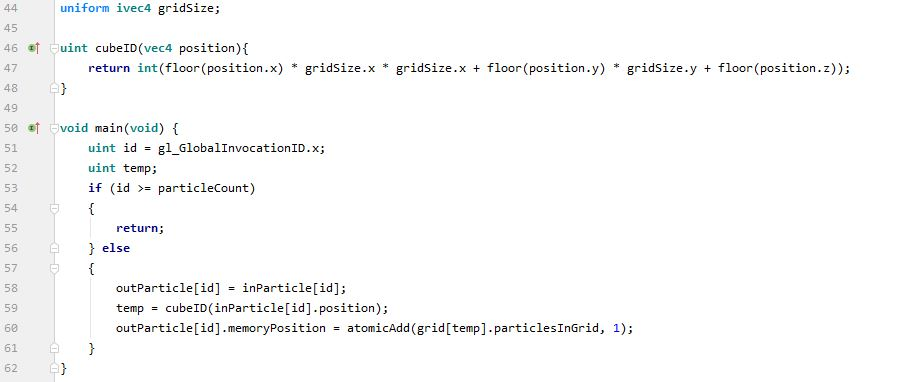
\includegraphics[width=1.3\columnwidth]{Bilder/lable.jpg}
	\caption{registrieren der Partikel im Grid mit CubeID-Funktion }
	\label{img:lable}
\end{figure}

 Dabei wird wie in Abbildung \ref{img:lable} in Zeile 60 zu sehen die Anzahl der Partikel in einem Gridbehälter gespeichtert. Die atomicAdd-Funktion wird dabei durchgeführt und es wird der Wert $grid[temp].particlesInGrid$ um 1 erhöht. 

%-------------------------------------------------------------------------------

\subsection{Vergleich}\label{vergleich}

%-------------------------------------------------------------------------------

\section{Ergebnis}\label{ergebnis}

%-------------------------------------------------------------------------------

\section{Fazit}\label{fazit}

%-------------------------------------------------------------------------------

%-------------------------------------------------------------------------------

\newpage
\listoffigures
\newpage
\bibliography{lib}

\end{document}